\begin{refsection}[research/kuramashi/group.bib]
\nocite{*}
\chapter{Field Theory Research Team}

\section{Members}

\begin{itemize}
  \item[] Yoshinobu Kuramashi (Team Leader)
  \item[] Yoshifumi Nakamura (Research Scientist)
  \item[] Hiroya Suno (Research Scientist, Joint Position with the Nishina Center for Accelerator-based Research)
  \item[] Eigo Shintani (Research Scientist)
  \item[] Yuya Shimizu (Postdoctoral Researcher)
  \item[] Yusuke Yoshimura (Postdoctoral Researcher)
  \item[] Ken-Ichi Ishikawa (Visiting Scientist, Hiroshima University)
  \item[] Takeshi Yamazaki (Visiting Scientist, University of Tsukuba)
  \item[] Shinji Takeda (Visiting Scientist, Kanazawa University)
\end{itemize}

\section{Research Activities}

 Our research field is physics of elementary particles and nuclei, which tries to answer questions in history of mankind: What is the smallest component of matter and what is the most fundamental interactions? This research subject is related to the early universe and the nucleosynthesis through Big Bang cosmology. Another important aspect is quantum properties, which play an essential role in the world of elementary particles and nuclei as well as in the material physics at the atomic or molecular level. We investigate nonperturbative properties of elementary particles and nuclei through numerical simulations with the use of lattice QCD (Quantum ChromoDynamics). The research is performed in collaboration with applied mathematicians, who are experts in developing and improving algorithms, and computer scientists responsible for research and development of software and hardware systems. 
   
 Lattice QCD is one of the most advanced case in quantum sciences: Interactions between quarks, which are elementary particles known to date, are described by QCD formulated with the quantum field theory. We currently focus on two research subjects: (1) QCD at finite temperature and finite density. We try to understand the early universe and the inside of neutron star by investigating the phase structure and the equation of state. (2) First principle calculation of nuclei based on QCD. Nuclei are bound states of protons and neutrons which consist of three quarks. We investigate the hierarchical structure of nuclei through the direct construction of nuclei in terms of quarks. 
     
 Successful numerical simulations heavily depend on an increase of computer performance by improving algorithms and computational techniques. However, we now face a tough problem that the trend of computer architecture becomes large-scale hierarchical parallel structures consisting of tens of thousands of nodes which individually have increasing number of cores in CPU and arithmetic accelerators with even higher degree of parallelism: We need to develop a new type of algorithms and computational techniques, which should be different from the conventional ones, to achieve better computer performance. For optimized use of K computer our research team aims at (1) developing a Monte Carlo algorithm to simulate physical system with negative weight effectively and (2) improving iterative methods to solve large system of linear equations. These technical development and improvement are carried out in the research of physics of elementary particles and nuclei based on lattice QCD.

\section{Research Results and Achievements}


%\begin{figure}
%\centering
%  \includegraphics[width=0.5\textwidth,keepaspectratio,natwidth=193,natheight=40]
%  {sample_division/sample_group/test1.png}
%  \caption{Caption for a sample figure}
%  \locallabel{fig:sample-label1}
%\end{figure}

\subsection{QCD at finite temperature and finite density}

Establishing the QCD phase diagram spanned by the temperature $T$ and the quark chemical potential $\mu$ in a quantitative way is an important task of lattice QCD. We have been working on tracing the critical end line in the parameter space of temperature, chemical potential and quark masses in 3 and 2+1 flavor QCD using the $O(a)$-improved Wilson quark action and the Iwasaki gauge action. As a first step we have determined the critical end point at zero chemical potential $\mu=0$ in 3 flavor case. Our strategy is to identify at which temperature the Kurtosis of physical observable measured at the transition point on several different spatial volumes intersects. This method is based on the property of opposite spatial volume dependences of the Kurtosis at the transition point between the first order phase transition side and the crossover one. We have obtained $T_{\rm E}$=133(2)(1)(3) MeV and $m_{\rm PS,E}$=306(7)(14)(7) MeV for the temperature and the pseudoscalar meson mass at the critical end point. This is the world's first determination of the critical end point in 3 flavor QCD providing a significant step forward in our understanding of the phase diagram. As a next step we have investigated the phase structure in the presence of finite chemical potential $\mu\ne 0$ in 3 flavor QCD\cite{cel_3f}. We have successfully determined the curvature of the critical end line on the $\mu/T$-$(m_{\rm PS})^2$ plane near the vanishing chemical potential employing the Kurtosis intersection method and the multi-parameter reweighting method. After the investigation with and without the chemical potential in 3 flavor QCD, we  embark on the determination of the critical end line of the finite temperature phase transition in 2+1 flavor QCD. We first focus on the behavior of the critical end line around the SU(3) symmetric point ($m_{\rm ud}=m_{\rm s}$) at the temporal size $N_T=6$ with the lattice spacing as low as $a\approx 0.19$ fm\cite{cel_2+1f}.
Figure~\localref{fig:cel} plots the critical end line on the $m_\pi^2$-$m_{\eta_s}^2$ plane, where the pink line indicates $m_{\rm ud}=m_{\rm s}$ ($m_\pi=m_{\eta_s}$). We confirm that the slope of the critical end line takes the value of $-2$ at the SU(3) symmetric point, and find that the second derivative is positive. At present our investigation is extended to  wider range of quark masses away from the SU(3) symmetric point.  

 \begin{figure}
\centering
 % \includegraphics[width=0.5\textwidth,keepaspectratio,natwidth=193,natheight=40]
 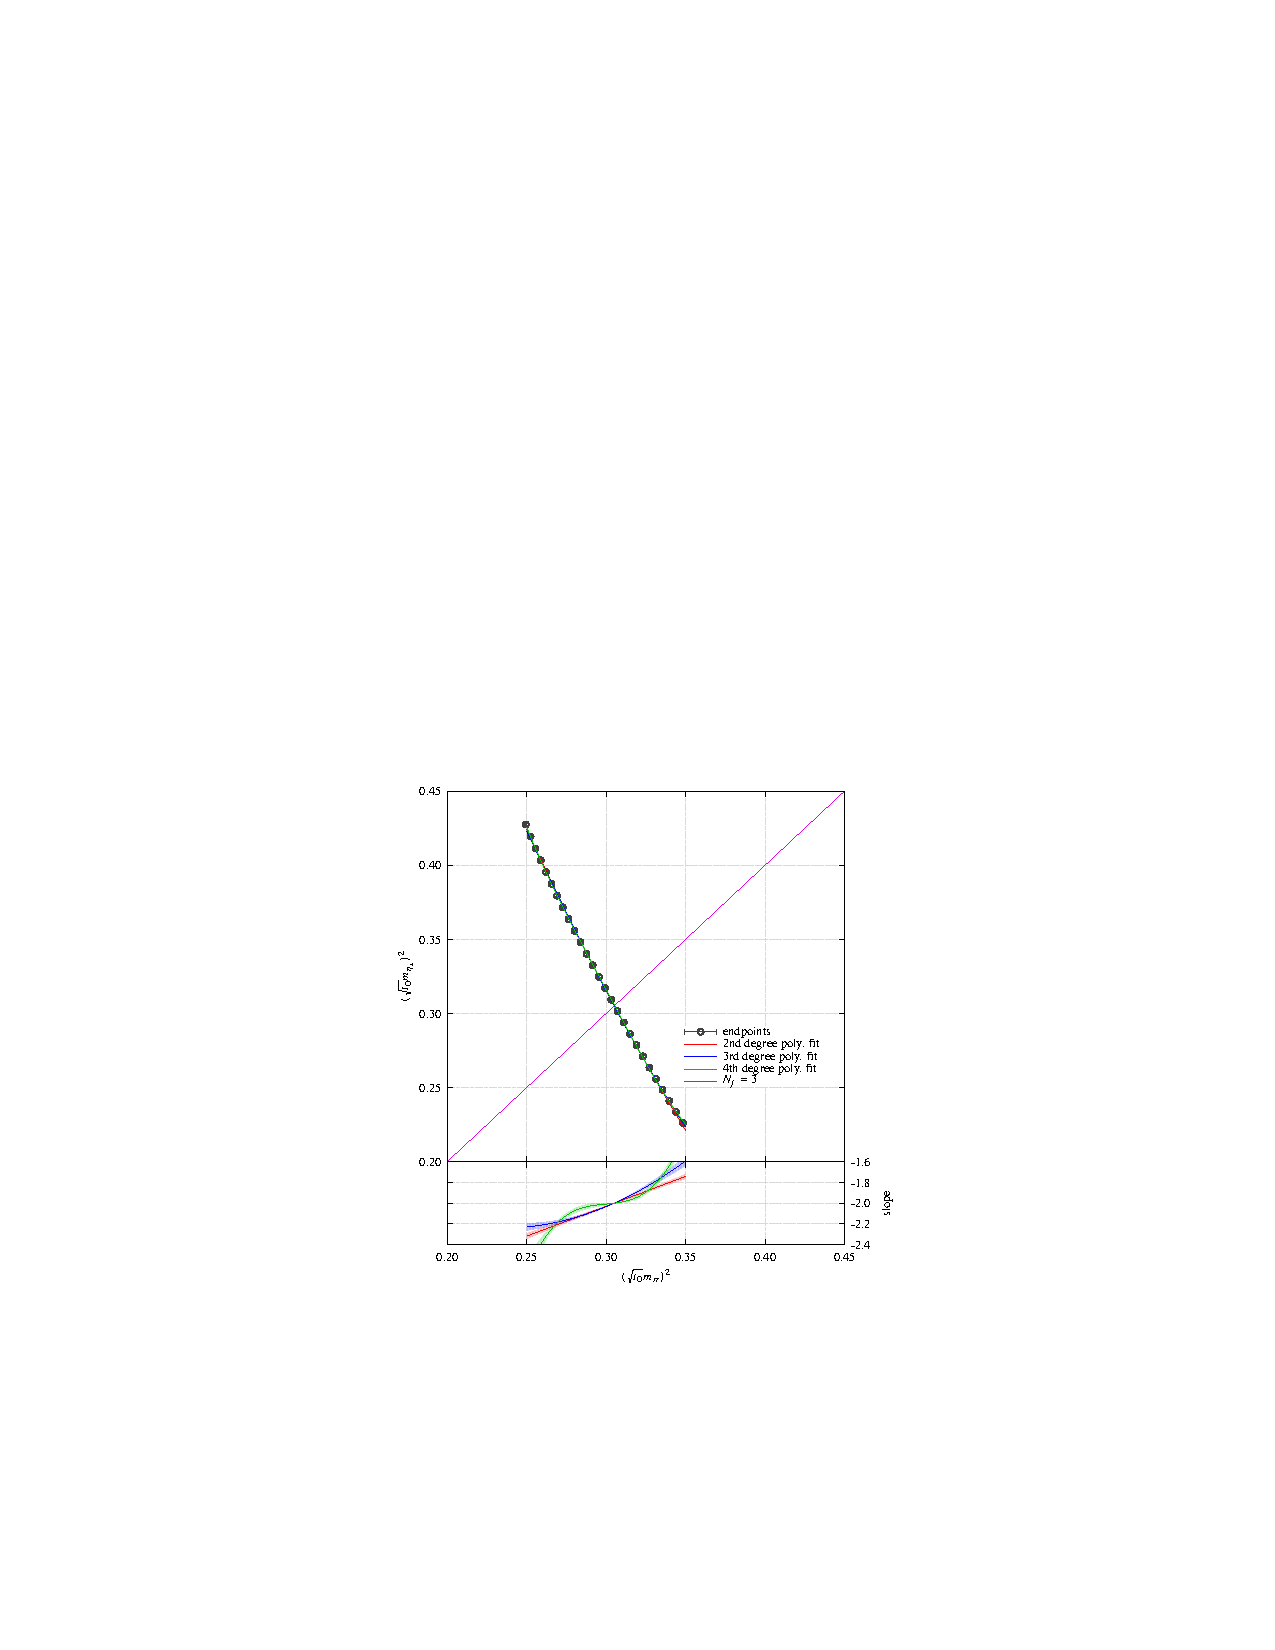
\includegraphics[width=100mm]{research/kuramashi/figs/cel.pdf} 
  \caption{Critical end line on the $m_\pi^2$-$m_{\eta_s}^2$ plane (top) and the slope along the critical end line (bottom). $\sqrt{t_0}$ denotes the Wilson flow scale.}
  \locallabel{fig:cel}
\end{figure}

\subsection{Nuclei in lattice QCD}

In 2010 we succeeded in a direct construction of the ${}^4$He and ${}^3$He nuclei from quarks and gluons in lattice QCD for the first time in the world. Calculations were carried out at a rather heavy degenerate up and down quark mass corresponding to $m_\pi$=0.8 GeV in quenched QCD to control statistical errors in the Monte Carlo evaluation of the helium Green functions. As a next step we investigated the dynamical quark effects on the binding energies of the helium nuclei, the deuteron and the dineutron. We performed a 2+1 flavor lattice QCD simulation with the degenerate up and down quark mass corresponding to $m_\pi$=0.51 GeV. To distinguish a bound state from an attractive scattering state, we investigate the spatial volume dependence of the energy difference between the ground state and the free multi-nucleon state by changing the spatial extent of the lattice from 2.9 fm to 5.8 fm. We observed that the measured ground states for all the channels are bound. This result raises an issue concerning the quark mass dependence. At the physical quark mass, namely in experiment, there is no bound state in the dineutron channel. So we expect that the bound state in the dineutron channel observed in our simulation at $m_\pi$=0.51 GeV may disappear at some quark mass toward the physical value. A new simulation at $m_\pi$=0.30 GeV, however,  reveals that the ground states in all channels are bound states showing rather weak quark mass dependence in the region from $m_\pi$=0.30 GeV to 0.51 GeV\cite{nuclei_mpi300}. In order to understand the quark mass dependence more systematically, we are currently working on the calculation of the binding energies for the helium nuclei, the deuteron and the dineutron at the physical point on a $96^4$ lattice.  Figure~\localref{fig:dE_3he} shows a preliminary result for the effective energy difference of ${}^3$He nuclei, which should represent the binding energy in large time region. Although the statistical precision is not sufficient at this stage, we plan to diminish the error bars with increasing statistics. 

 \begin{figure}
\centering
 % \includegraphics[width=0.5\textwidth,keepaspectratio,natwidth=193,natheight=40]
 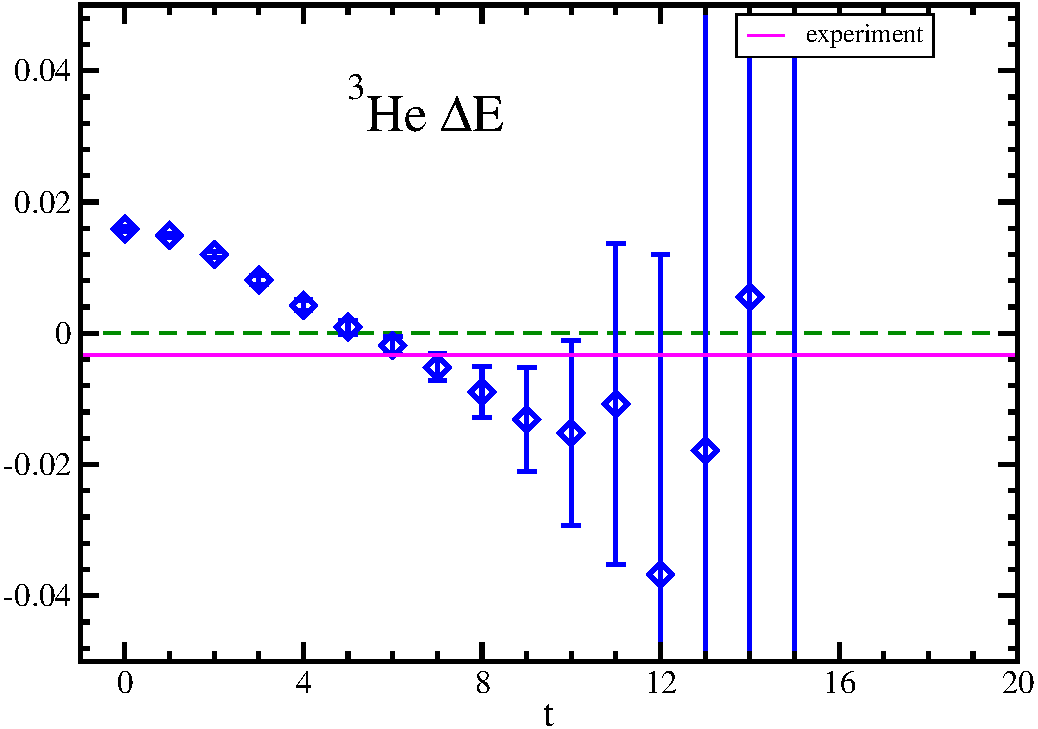
\includegraphics[width=100mm]{research/kuramashi/figs/dE_3he.pdf} 
  \caption{Effective energy difference for ${}^3$He nuclei as a function of time. Solid line indicates the experimental result for the binding energy.}
  \locallabel{fig:dE_3he}
\end{figure}

\subsection{Development of algorithms and computational techniques}

\subsubsection{Application of z-Pares to lattice QCD on K computer}

Eigenvalue problem for a given large sparse matrix is common across various computational sciences including lattice QCD. Sakurai group in University of Tsukuba, who has been working on the eigenvalue problem for sparse matrices for a long time, is now developing a software package for massively parallel eigenvalue computation for sparse matrices called z-Pares (short for Complex Moment-based Parallel Eigen-Solvers). We have applied z-Pares to a large scale calculation of lattice QCD on K computer. We need to solve the Wilson-Dirac equation $D{\vec x}={\vec b}$ in lattice QCD, where $D$ is an $N\times N$ complex sparse non-Hermitian matrix with $N$ the number of four dimensional space-time sites multiplied by 12. In current typical simulations the dimension $N$ is $O(10^9)$. z-Pares implements a complex moment based contour integral eigensolver: It computes eigenvalues inside a user-specified discretized contour path on the complex plane and corresponding eigenvectors. In most cases of lattice QCD calculations our interest is restricted to $O(10)$ eigenvalues around the origin so that lattice QCD should be a good example of application of z-Pares. Figure~\localref{fig:zpares_free} shows a test study comparing the analytic results (black crosses) and the numerical ones (red circles) for the eigenvalues of the free (without interactions with gauge fields) Wilson-Dirac matrix on a $96^4$ lattice. We observe both results show good agreement inside the contour. In Fig.~\localref{fig:zpares_full} we plot the numerical results for the eigenvalues of the $O(a)$-improved Wilson-Dirac matrix on a $96^4$ lattice used for a state-of-the-art calculation in lattice QCD, whose configuration properties are explained in Ref.~\cite{lat15_075}. We find four eigenvalues (red circles) near the origin. We are now working on an algorithmic improvement to efficiently solve the shifted Wilson-Dirac equation on the discretized contour. 
 
 \begin{figure}
\centering
 % \includegraphics[width=0.5\textwidth,keepaspectratio,natwidth=193,natheight=40]
 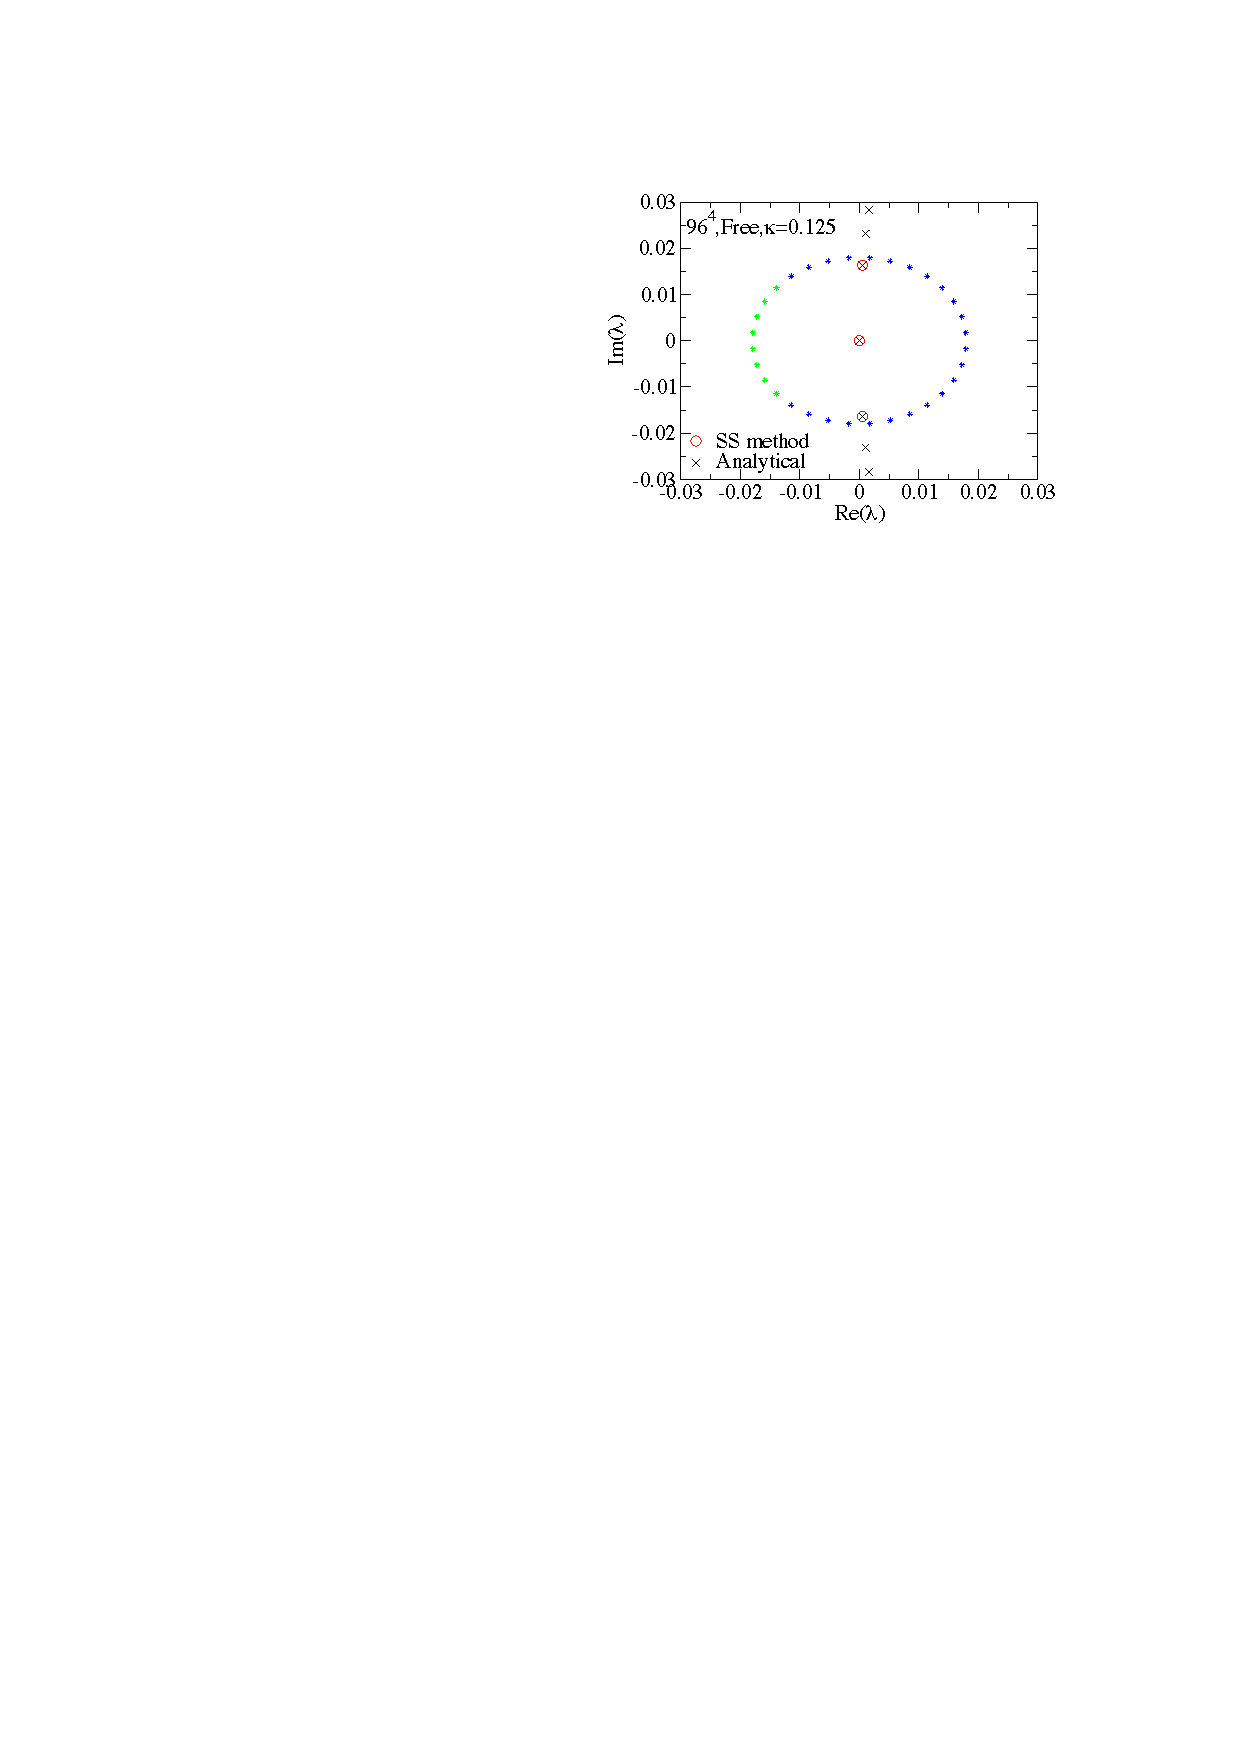
\includegraphics[width=100mm]{research/kuramashi/figs/zpares_free.pdf} 
  \caption{Eigenvalue distribution of the free (without interactions with gauge fields) Wilson-Dirac matrix on a $96^4$ lattice. $\kappa$ is a parameter to control the mass of the Wilson quark. Green and Blue star symbols denote the discretized contour around the origin of the complex plane. Black crosses denote the analytic results for the eigenvalues and red circles is for the numerical ones obtained by z-Pares.}
  \locallabel{fig:zpares_free}
\end{figure}

 \begin{figure}
\centering
 % \includegraphics[width=0.5\textwidth,keepaspectratio,natwidth=193,natheight=40]
 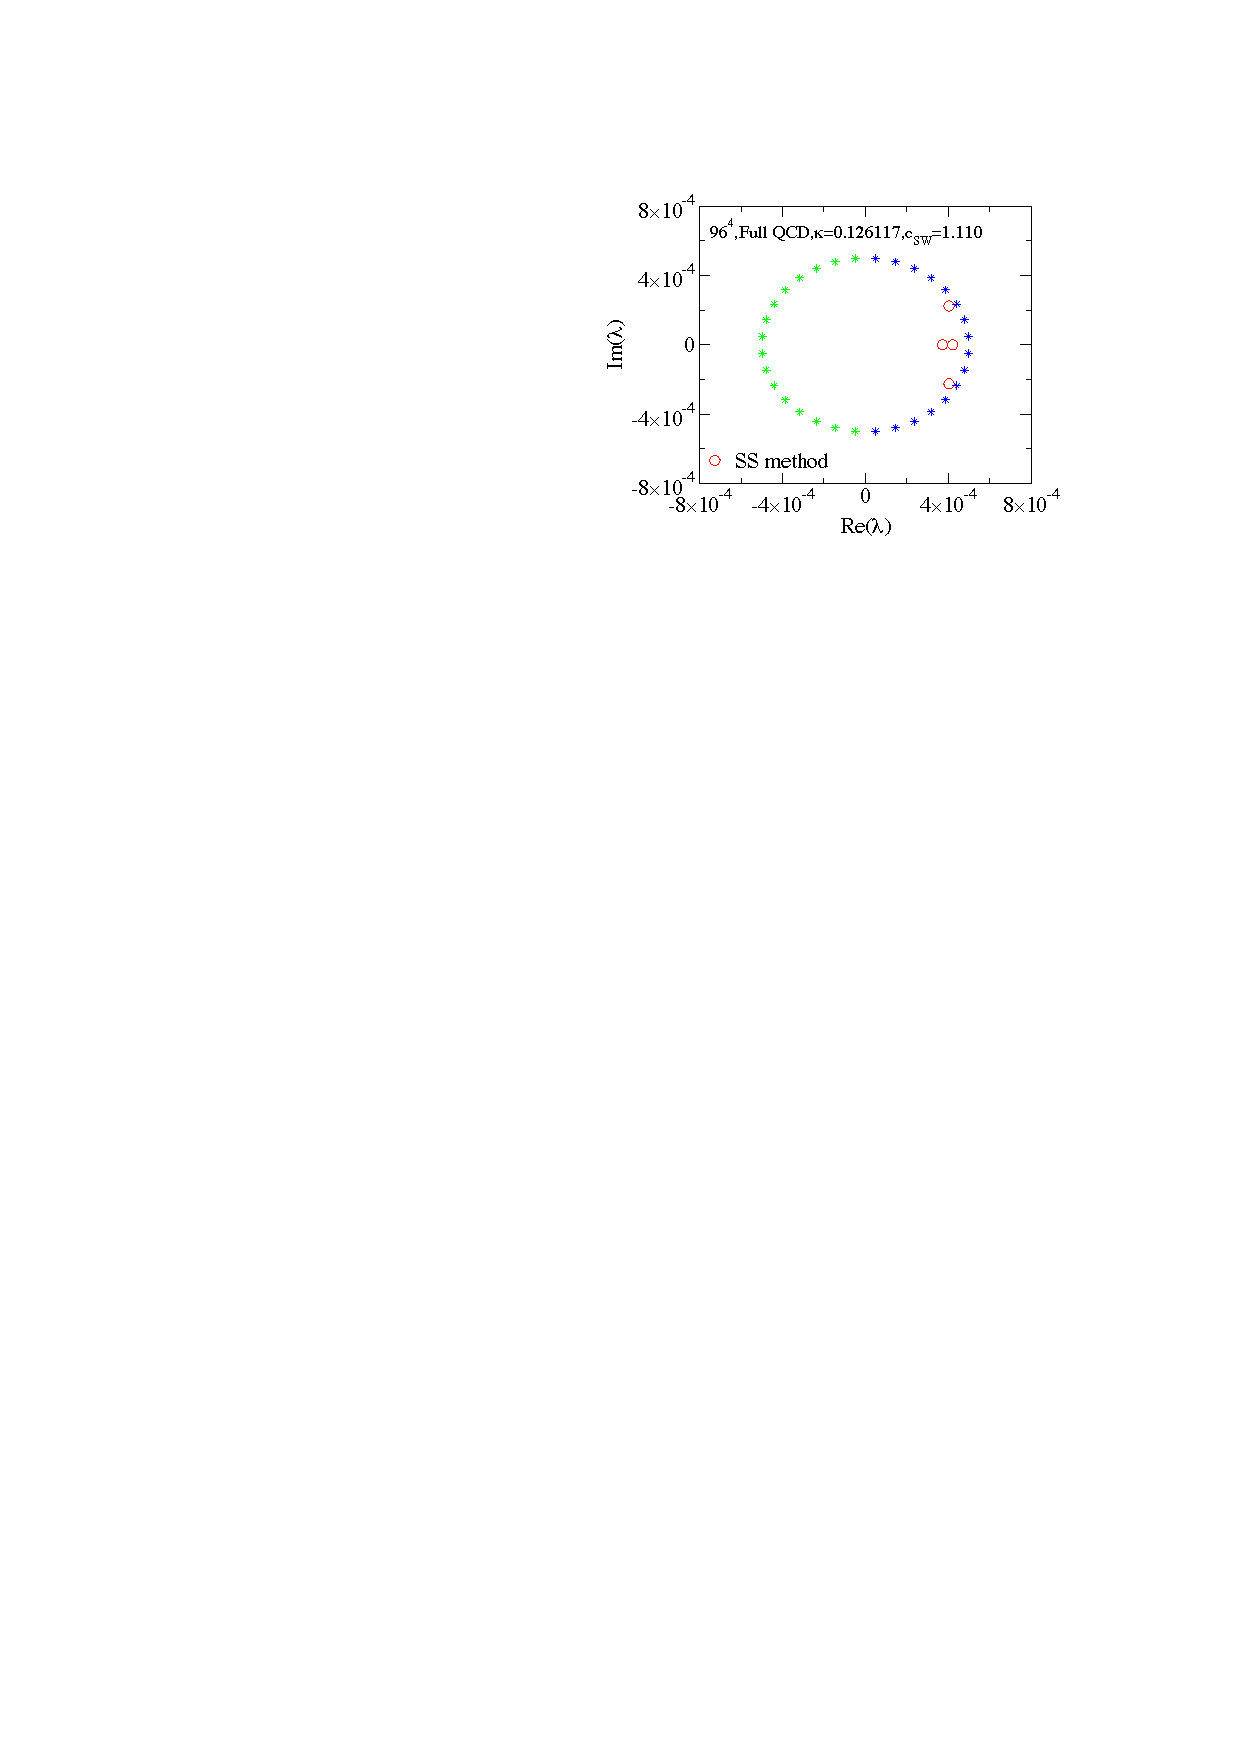
\includegraphics[width=100mm]{research/kuramashi/figs/zpares_full.pdf} 
  \caption{Same as Fig.~\protect{\localref{fig:zpares_free}} for the $O(a)$-improved Wilson-Dirac matrix in 2+1 flavor QCD.}
  \locallabel{fig:zpares_full}
\end{figure}

\subsubsection{Tensor network scheme in path-integral formalism}

The Monte Carlo simulation of lattice gauge theory is quite powerful to study nonperturbative phenomena of particle physics. However, when the action has an imaginary component like the $\theta$ term, it suffers from the numerical sign problem, failure of importance sampling techniques. The effect of the $\theta$ term on non-Abelian gauge theory, especially quantum chromodynamics (QCD) is important, because it is related to a famous unsolved problem, ``strong CP problem''. The difficulty is also shared with finite density lattice QCD. So development of effective techniques to solve or by-pass the sign problem leads to a lot of progress in the study of the QCD phase diagram at finite temperature and density. The tensor network scheme is a promising theoretical and computational framework to overcome these difficulties. So far we have developed the Grassmann version of the tensor renormalization group (GTRG) algorithm in the tensor network scheme, which allows us to deal with the Grassmann variables directly. The GTRG algorithm was successfully applied to the analysis on the phase structure of one-flavor lattice Schwinger model (2D QED) with and without the $\theta$ term showing that the algorithm is free from the sign problem and the computational cost is comparable to the bosonic case thanks to the direct manipulation of the Grassmann variables. This was the first successful application of the tensor network scheme to a Euclidean lattice gauge theory including relativistic fermions. Toward the final target of 4D QCD we are currently working on three research subjects in the tensor network scheme: (i) non-Abelian gauge theories, (ii) higher dimensional (3D or 4D) models, and (iii) development of computational techniques for physical observables.  Figure~\localref{fig:kc_dcut} presents a preliminary result for analysis of the phase transition in the 4D Ising model. The precision of the GTRG algorithm is controlled by the parameter $D_{\rm cut}$. We observe that the critical (inverse) temperature $K_{\rm c}$ converges close to the previous Monte Carlo result (blue line) as $D_{\rm cut}$ increases. It should be noted that our result is directly obtained on a $1024^4$ lattice, while the Monte Carlo result was obtained by extrapolating the data on $80^4$ and smaller lattices to the thermodynamic limit. 

 \begin{figure}
\centering
 % \includegraphics[width=0.5\textwidth,keepaspectratio,natwidth=193,natheight=40]
 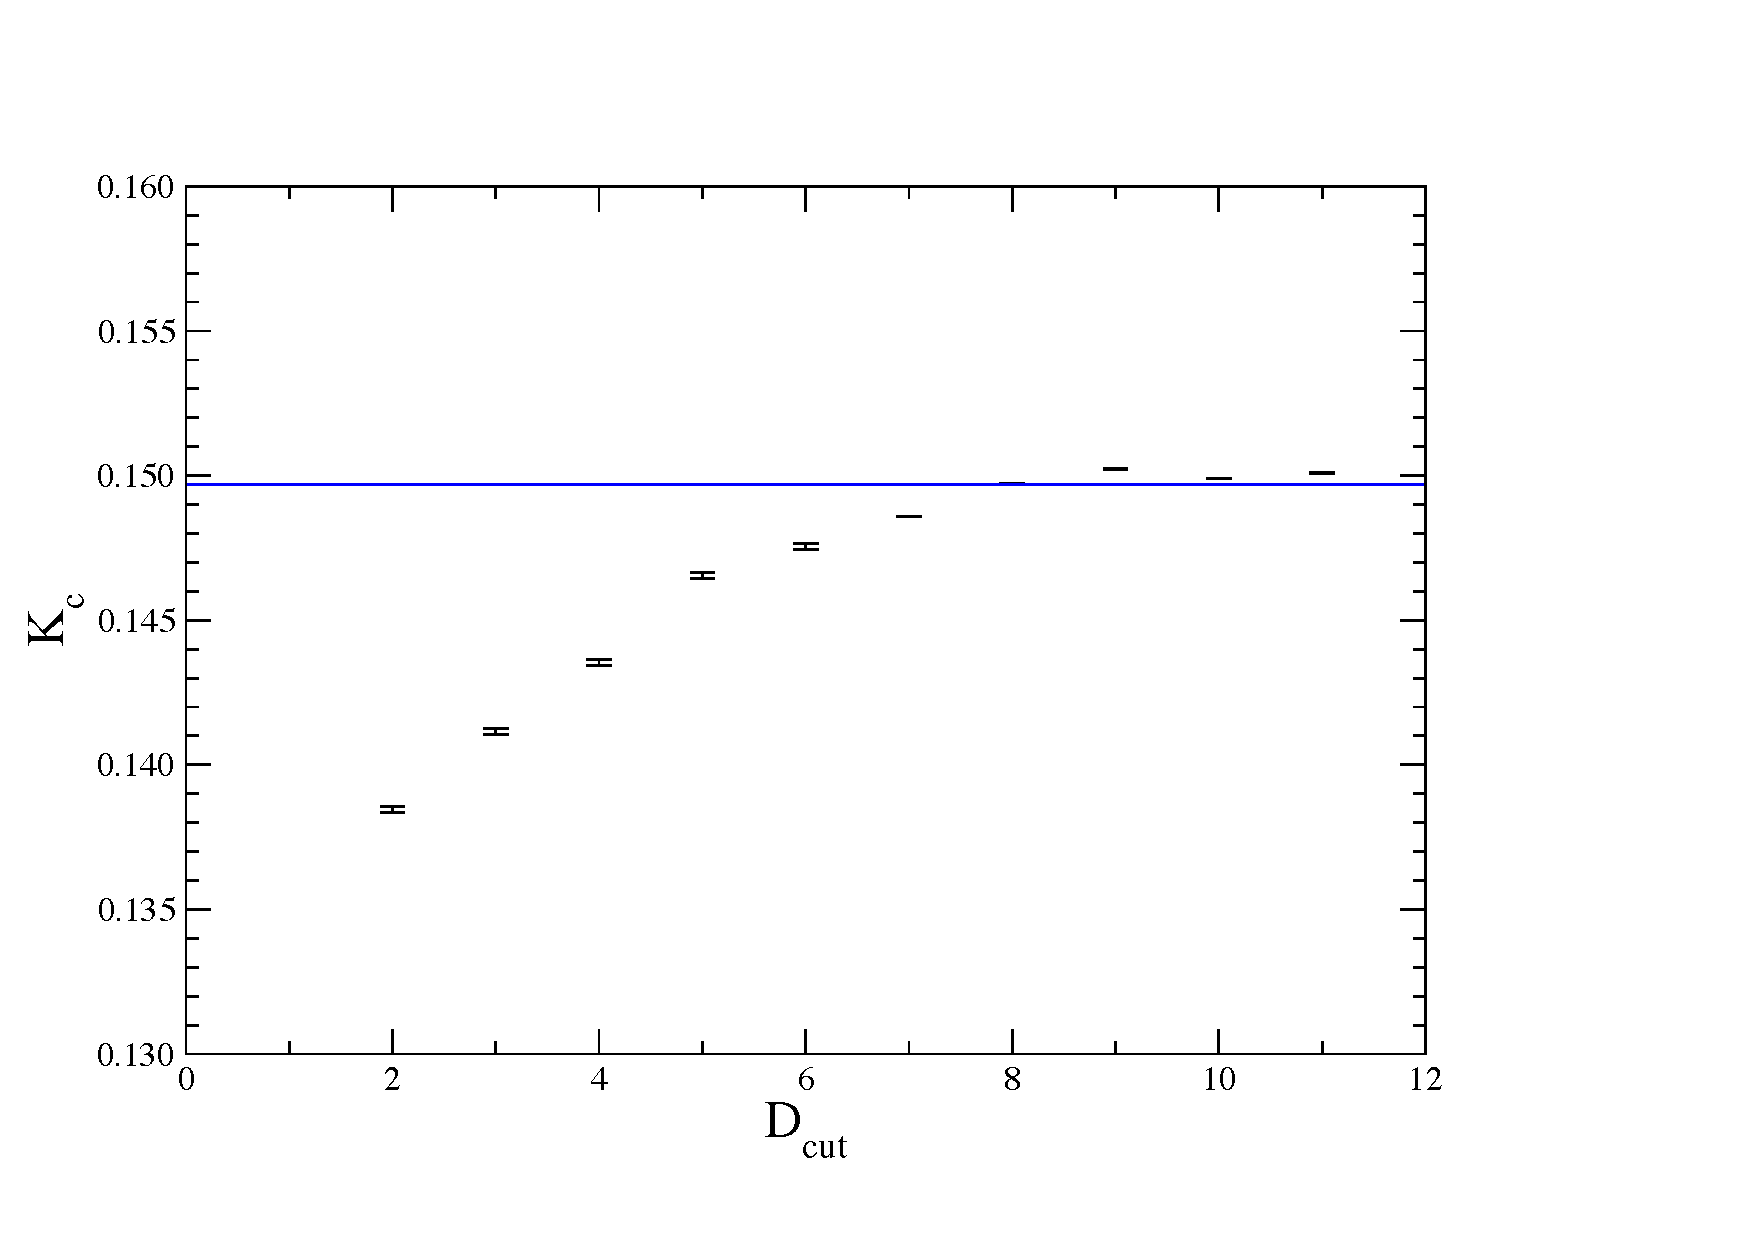
\includegraphics[width=100mm]{research/kuramashi/figs/kc_dcut.pdf} 
  \caption{$D_{\rm cut}$ dependence of critical (inverse) temperature $K_{\rm c}$ in 4D Ising model on a $1024^4$ lattice. Blue line denotes the previous Monte Carlo result.}
  \locallabel{fig:kc_dcut}
\end{figure}

\section{Schedule and Future Plan}

\subsection{QCD at finite temperature and finite density}

We are now investigating the phase structure in 2+1 flavor QCD with the Kurtosis intersection method and the multi-parameter reweighting method. The first target is to determine the critical end line on the $m_{\rm ud}$-$m_{\rm s}$ plane. Especially, we are interested in small $m_{\rm ud}$ region. 

\subsection{Nuclei in lattice QCD}

So far our study reveals that the dineutron channel is a bound state at heavier quark masses corresponding to $m_{\pi}\ge 300$ MeV. We currently make a large scale simulation at the physical quark mass. We are also investigating possible sources of the systematic errors.  

\subsection{Development of algorithms and computational techniques}

\subsubsection{Application of z-Pares to lattice QCD on K computer}

In collaboration with Sakurai group at University of Tsukuba  we work on an algorithmic improvement to efficiently solve the shifted Wilson-Dirac equation on the discretized contour. 

\subsubsection{Tensor network scheme in path-integral formalism}

We are now try to apply the tensor network scheme to various spin models and  non-Abelian lattice gauge theories on higher dimensions. It is also an interesting subject to apply the GTRG method to the chiral fermion. 

%%% DO NOT EDIT BELOW

\section{Publications}

%\printbibliography[keyword=journal, heading=subbibliography, title={Journal Articles}, prefixnumbers={1-}, resetnumbers=true]
%\printbibliography[keyword=proceedings, heading=subbibliography, title={Conference Papers}, prefixnumbers={2-}, resetnumbers=true]
%\printbibliography[keyword=invited, heading=subbibliography, title={Invited Talks}, prefixnumbers={3-}, resetnumbers=true]
%\printbibliography[keyword=poster, heading=subbibliography, title={Posters and Presentations}, prefixnumbers={4-}, resetnumbers=true]
%\printbibliography[keyword=deliverable, heading=subbibliography, title={Patents and Deliverables}, prefixnumbers={5-}, resetnumbers=true]

\printbibliography[keyword=journal, heading=subbibliography, title={Journal Articles}, resetnumbers=true]
\printbibliography[keyword=proceedings, heading=subbibliography, title={Conference Papers}]
\printbibliography[keyword=invited, heading=subbibliography, title={Invited Talks}]
\printbibliography[keyword=poster, heading=subbibliography, title={Posters and Presentations}]
\printbibliography[keyword=deliverable, heading=subbibliography, title={Patents and Deliverables}]

\end{refsection}
